
%% bare_conf.tex 
%% V1.2
%% 2002/11/18
%% by Michael Shell
%% mshell@ece.gatech.edu
%% 
%% NOTE: This text file uses MS Windows line feed conventions. When (human)
%% reading this file on other platforms, you may have to use a text
%% editor that can handle lines terminated by the MS Windows line feed
%% characters (0x0D 0x0A).
%% 
%% This is a skeleton file demonstrating the use of IEEEtran.cls 
%% (requires IEEEtran.cls version 1.6b or later) with an IEEE conference paper.
%% 
%% Support sites:
%% http://www.ieee.org
%% and/or
%% http://www.ctan.org/tex-archive/macros/latex/contrib/supported/IEEEtran/ 
%%
%% This code is offered as-is - no warranty - user assumes all risk.
%% Free to use, distribute and modify.

% *** Authors should verify (and, if needed, correct) their LaTeX system  ***
% *** with the testflow diagnostic prior to trusting their LaTeX platform ***
% *** with production work. IEEE's font choices can trigger bugs that do  ***
% *** not appear when using other class files.                            ***
% Testflow can be obtained at:
% http://www.ctan.org/tex-archive/macros/latex/contrib/supported/IEEEtran/testflow


% Note that the a4paper option is mainly intended so that authors in
% countries using A4 can easily print to A4 and see how their papers will
% look in print. Authors are encouraged to use U.S. letter paper when 
% submitting to IEEE. Use the testflow package mentioned above to verify
% correct handling of both paper sizes by the author's LaTeX system.
%
% Also note that the "draftcls" or "draftclsnofoot", not "draft", option
% should be used if it is desired that the figures are to be displayed in
% draft mode.
%
% This paper can be formatted using the peerreviewca
% (instead of conference) mode.
\documentclass[conference]{IEEEtran}
% If the IEEEtran.cls has not been installed into the LaTeX system files, 
% manually specify the path to it:
% \documentclass[conference]{../sty/IEEEtran} 


% some very useful LaTeX packages include:
\usepackage{array}
\newcolumntype{C}[1]{>{\centering\arraybackslash}p{#1}}

\usepackage{cite}      % Written by Donald Arseneau
                        % V1.6 and later of IEEEtran pre-defines the format
                        % of the cite.sty package \cite{} output to follow
                        % that of IEEE. Loading the cite package will
                        % result in citation numbers being automatically
                        % sorted and properly "ranged". i.e.,
                        % [1], [9], [2], [7], [5], [6]
                        % (without using cite.sty)
                        % will become:
                        % [1], [2], [5]--[7], [9] (using cite.sty)
                        % cite.sty's \cite will automatically add leading
                        % space, if needed. Use cite.sty's noadjust option
                        % (cite.sty V3.8 and later) if you want to turn this
                        % off. cite.sty is already installed on most LaTeX
                        % systems. The latest version can be obtained at:
                        % http://www.ctan.org/tex-archive/macros/latex/contrib/supported/cite/

\usepackage{graphicx}  % Written by David Carlisle and Sebastian Rahtz
 \usepackage{tabu}                       % Required if you want graphics, photos, etc.
                        % graphicx.sty is already installed on most LaTeX
                        % systems. The latest version and documentation can
                        % be obtained at:
                        % http://www.ctan.org/tex-archive/macros/latex/required/graphics/
                        % Another good source of documentation is "Using
                        % Imported Graphics in LaTeX2e" by Keith Reckdahl
                        % which can be found as esplatex.ps and epslatex.pdf
                        % at: http://www.ctan.org/tex-archive/info/
% NOTE: for dual use with latex and pdflatex, instead load graphicx like:
%\ifx\pdfoutput\undefined
%\usepackage{graphicx}
%\else
%\usepackage[pdftex]{graphicx}
%\fi

% However, be warned that pdflatex will require graphics to be in PDF
% (not EPS) format and will preclude the use of PostScript based LaTeX
% packages such as psfrag.sty and pstricks.sty. IEEE conferences typically
% allow PDF graphics (and hence pdfLaTeX). However, IEEE journals do not
% (yet) allow image formats other than EPS or TIFF. Therefore, authors of
% journal papers should use traditional LaTeX with EPS graphics.
%
% The path(s) to the graphics files can also be declared: e.g.,
% \graphicspath{{../eps/}{../ps/}}
% if the graphics files are not located in the same directory as the
% .tex file. This can be done in each branch of the conditional above
% (after graphicx is loaded) to handle the EPS and PDF cases separately.
% In this way, full path information will not have to be specified in
% each \includegraphics command.
%
% Note that, when switching from latex to pdflatex and vice-versa, the new
% compiler will have to be run twice to clear some warnings.


%\usepackage{psfrag}    % Written by Craig Barratt, Michael C. Grant,
                        % and David Carlisle
                        % This package allows you to substitute LaTeX
                        % commands for text in imported EPS graphic files.
                        % In this way, LaTeX symbols can be placed into
                        % graphics that have been generated by other
                        % applications. You must use latex->dvips->ps2pdf
                        % workflow (not direct pdf output from pdflatex) if
                        % you wish to use this capability because it works
                        % via some PostScript tricks. Alternatively, the
                        % graphics could be processed as separate files via
                        % psfrag and dvips, then converted to PDF for
                        % inclusion in the main file which uses pdflatex.
                        % Docs are in "The PSfrag System" by Michael C. Grant
                        % and David Carlisle. There is also some information 
                        % about using psfrag in "Using Imported Graphics in
                        % LaTeX2e" by Keith Reckdahl which documents the
                        % graphicx package (see above). The psfrag package
                        % and documentation can be obtained at:
                        % http://www.ctan.org/tex-archive/macros/latex/contrib/supported/psfrag/

%\usepackage{subfigure} % Written by Steven Douglas Cochran
                        % This package makes it easy to put subfigures
                        % in your figures. i.e., "figure 1a and 1b"
                        % Docs are in "Using Imported Graphics in LaTeX2e"
                        % by Keith Reckdahl which also documents the graphicx
                        % package (see above). subfigure.sty is already
                        % installed on most LaTeX systems. The latest version
                        % and documentation can be obtained at:
                        % http://www.ctan.org/tex-archive/macros/latex/contrib/supported/subfigure/

%\usepackage{url}       % Written by Donald Arseneau
                        % Provides better support for handling and breaking
                        % URLs. url.sty is already installed on most LaTeX
                        % systems. The latest version can be obtained at:
                        % http://www.ctan.org/tex-archive/macros/latex/contrib/other/misc/
                        % Read the url.sty source comments for usage information.

%\usepackage{stfloats}  % Written by Sigitas Tolusis
                        % Gives LaTeX2e the ability to do double column
                        % floats at the bottom of the page as well as the top.
                        % (e.g., "\begin{figure*}[!b]" is not normally
                        % possible in LaTeX2e). This is an invasive package
                        % which rewrites many portions of the LaTeX2e output
                        % routines. It may not work with other packages that
                        % modify the LaTeX2e output routine and/or with other
                        % versions of LaTeX. The latest version and
                        % documentation can be obtained at:
                        % http://www.ctan.org/tex-archive/macros/latex/contrib/supported/sttools/
                        % Documentation is contained in the stfloats.sty
                        % comments as well as in the presfull.pdf file.
                        % Do not use the stfloats baselinefloat ability as
                        % IEEE does not allow \baselineskip to stretch.
                        % Authors submitting work to the IEEE should note
                        % that IEEE rarely uses double column equations and
                        % that authors should try to avoid such use.
                        % Do not be tempted to use the cuted.sty or
                        % midfloat.sty package (by the same author) as IEEE
                        % does not format its papers in such ways.

%\usepackage{amsmath}   % From the American Mathematical Society
                        % A popular package that provides many helpful commands
                        % for dealing with mathematics. Note that the AMSmath
                        % package sets \interdisplaylinepenalty to 10000 thus
                        % preventing page breaks from occurring within multiline
                        % equations. Use:
%\interdisplaylinepenalty=2500
                        % after loading amsmath to restore such page breaks
                        % as IEEEtran.cls normally does. amsmath.sty is already
                        % installed on most LaTeX systems. The latest version
                        % and documentation can be obtained at:
                        % http://www.ctan.org/tex-archive/macros/latex/required/amslatex/math/



% Other popular packages for formatting tables and equations include:

%\usepackage{array}
% Frank Mittelbach's and David Carlisle's array.sty which improves the
% LaTeX2e array and tabular environments to provide better appearances and
% additional user controls. array.sty is already installed on most systems.
% The latest version and documentation can be obtained at:
% http://www.ctan.org/tex-archive/macros/latex/required/tools/

% Mark Wooding's extremely powerful MDW tools, especially mdwmath.sty and
% mdwtab.sty which are used to format equations and tables, respectively.
% The MDWtools set is already installed on most LaTeX systems. The lastest
% version and documentation is available at:
% http://www.ctan.org/tex-archive/macros/latex/contrib/supported/mdwtools/


% V1.6 of IEEEtran contains the IEEEeqnarray family of commands that can
% be used to generate multiline equations as well as matrices, tables, etc.


% Also of notable interest:

% Scott Pakin's eqparbox package for creating (automatically sized) equal
% width boxes. Available:
% http://www.ctan.org/tex-archive/macros/latex/contrib/supported/eqparbox/



% Notes on hyperref:
% IEEEtran.cls attempts to be compliant with the hyperref package, written
% by Heiko Oberdiek and Sebastian Rahtz, which provides hyperlinks within
% a document as well as an index for PDF files (produced via pdflatex).
% However, it is a tad difficult to properly interface LaTeX classes and
% packages with this (necessarily) complex and invasive package. It is
% recommended that hyperref not be used for work that is to be submitted
% to the IEEE. Users who wish to use hyperref *must* ensure that their
% hyperref version is 6.72u or later *and* IEEEtran.cls is version 1.6b 
% or later. The latest version of hyperref can be obtained at:
%
% http://www.ctan.org/tex-archive/macros/latex/contrib/supported/hyperref/
%
% Also, be aware that cite.sty (as of version 3.9, 11/2001) and hyperref.sty
% (as of version 6.72t, 2002/07/25) do not work optimally together.
% To mediate the differences between these two packages, IEEEtran.cls, as
% of v1.6b, predefines a command that fools hyperref into thinking that
% the natbib package is being used - causing it not to modify the existing
% citation commands, and allowing cite.sty to operate as normal. However,
% as a result, citation numbers will not be hyperlinked. Another side effect
% of this approach is that the natbib.sty package will not properly load
% under IEEEtran.cls. However, current versions of natbib are not capable
% of compressing and sorting citation numbers in IEEE's style - so this
% should not be an issue. If, for some strange reason, the user wants to
% load natbib.sty under IEEEtran.cls, the following code must be placed
% before natbib.sty can be loaded:
%
% \makeatletter
% \let\NAT@parse\undefined
% \makeatother
%
% Hyperref should be loaded differently depending on whether pdflatex
% or traditional latex is being used:
%
%\ifx\pdfoutput\undefined
%\usepackage[hypertex]{hyperref}
%\else
%\usepackage[pdftex,hypertexnames=false]{hyperref}
%\fi
%
% Pdflatex produces superior hyperref results and is the recommended
% compiler for such use.



% *** Do not adjust lengths that control margins, column widths, etc. ***
% *** Do not use packages that alter fonts (such as pslatex).         ***
% There should be no need to do such things with IEEEtran.cls V1.6 and later.


% correct bad hyphenation here
\hyphenation{op-tical net-works semi-conduc-tor IEEEtran}


\begin{document}

% paper title
\title{An FPGA Cluster for Real-Time \\ Parallel Human Genome Assembly}


% author names and affiliations
% use a multiple column layout for up to three different
% affiliations
\author{
\authorblockN{----------}
\authorblockA{---------------------\\
--------------------\\
---------------------}
}


% avoiding spaces at the end of the author lines is not a problem with
% conference papers because we don't use \thanks or \IEEEmembership


% for over three affiliations, or if they all won't fit within the width
% of the page, use this alternative format:
% 
%\author{\authorblockN{Michael Shell\authorrefmark{1},
%Homer Simpson\authorrefmark{2},
%James Kirk\authorrefmark{3}, 
%Montgomery Scott\authorrefmark{3} and
%Eldon Tyrell\authorrefmark{4}}
%\authorblockA{\authorrefmark{1}School of Electrical and Computer Engineering\\
%Georgia Institute of Technology,
%Atlanta, Georgia 30332--0250\\ Email: mshell@ece.gatech.edu}
%\authorblockA{\authorrefmark{2}Twentieth Century Fox, Springfield, USA\\
%Email: homer@thesimpsons.com}
%\authorblockA{\authorrefmark{3}Starfleet Academy, San Francisco, California 96678-2391\\
%Telephone: (800) 555--1212, Fax: (888) 555--1212}
%\authorblockA{\authorrefmark{4}Tyrell Inc., 123 Replicant Street, Los Angeles, California 90210--4321}}



% use only for invited papers
%\specialpapernotice{(Invited Paper)}

% make the title area
\maketitle

\begin{abstract}
This paper presents a pixel based comparison engine for the purpose of speeding up the DNA seqeuncing process. Using the innate parallelism of FPGA hardware with a highly parallel algorithm this paper shows that an important part of the sequencing processing can be laid off to a hardware acceleration cluster. A demonstration of this was provided on a small cluster of Altera DE0 devices, with comparison speeds reaching up to 23 Million base comparisons per second in simulation, while the practical application reached 1.6 Million base comparisons per second for read lengths of 50 base pairs. \end{abstract}

% no keywords

% For peer review papers, you can put extra information on the cover
% page as needed:
% \begin{center} \bfseries EDICS Category: 3-BBND \end{center}
%
% for peerreview papers, inserts a page break and creates the second title.
% Will be ignored for other modes.
\IEEEpeerreviewmaketitle



\section{Introduction}
% no \PARstart
DNA Sequencing has been an area of a large amount of research in recent years with a number of Next Generation Technologies significantly increasing the speed at which sequencing can be carried out. However, these techniques have a common bottle-neck due to the massively parallel approach of the detection technologies.  In order to allow for long seqeunces to be detected a number of tool-chains have been designed with complex digital processing back-ends. 

The most computationally intensive part of this task is often found to be the all-against-all of sub-seqeunces comparison needed for some algorithms. This task has an $O(n^2)$ complexity, making it scale poorly. 

Currently the primary algorithms used for the recombination process are CPU and GPU based, using large amounts of compute power often over clusters of machines to solve this issue. In this paper a new application of an existing comparison engine will be presented, using the parrallel nature of FPGA devices to speed-up the all-against-all comparison.

Section 2 will introduce the background of DNA sequencing in terms of the common methods used and the requirements these configurations put upon the comparison engines. Section 3 will then introduce a comparison engine algorithm that can be implemented in a massively parallel manner suitable for FPGA designs and highlights the key features which make this a pracitcal solution for high speed processing. This will then be expanded upon in section 4 introducing a new system design for implementing this algorithm on an FPGA cluster, modifying the core algorithm to meet the practical constraints of the FPGA hardware. Section 5 will then discuss a practical implementation of this system on a set oF Altera FPGAs used as a proof-of-concept. Section 6 will explore the performance characteristics of this design with particular focus put on the scalability of the design as well as core computational speed.
\begin{center}
\begin{figure*}
  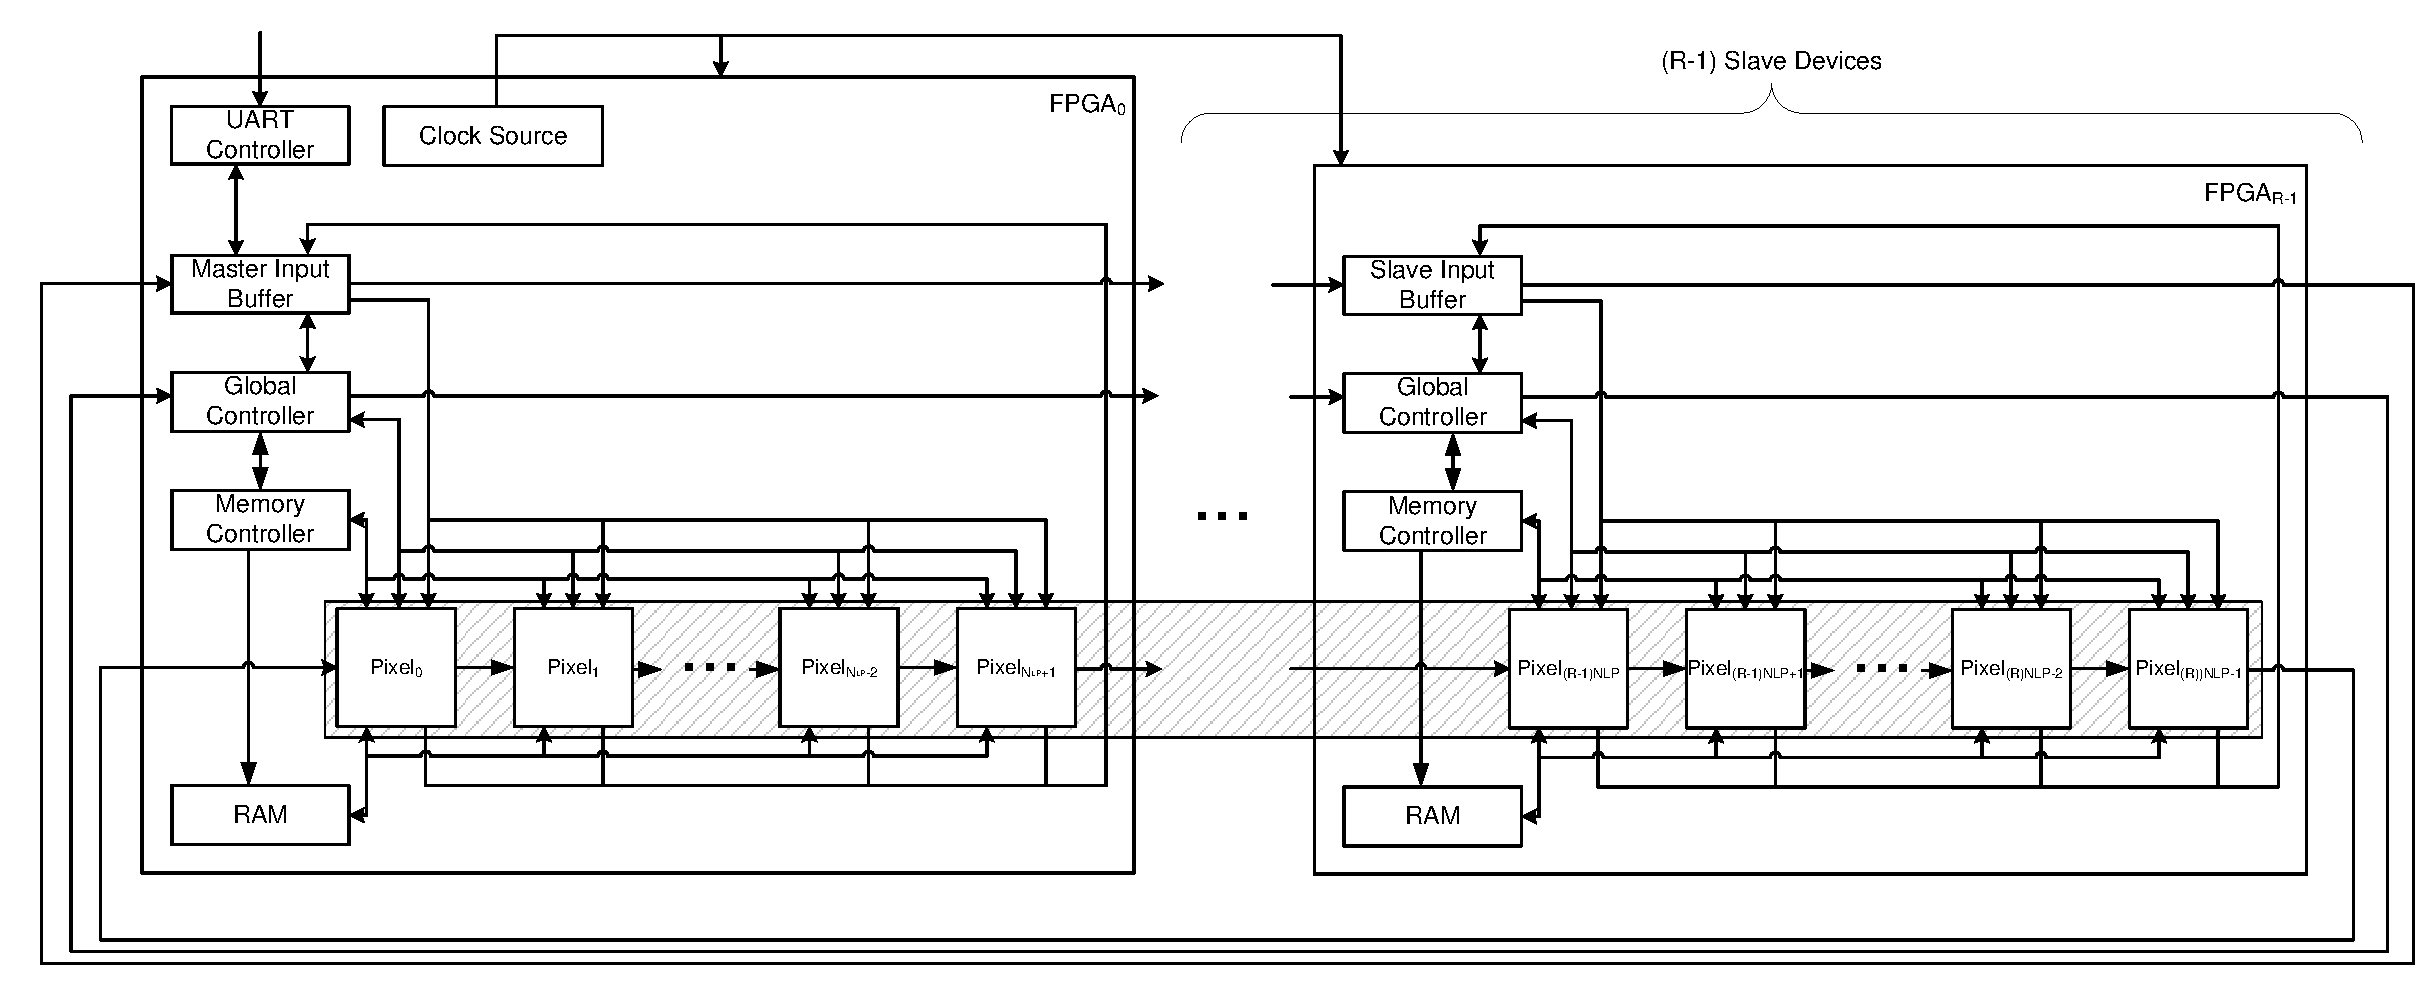
\includegraphics[width=\textwidth]{./figs/MFPGA.pdf}
  \caption{Top Level Diagram, 1 Host, R-1 Slave Devices}
  \label{fig:tld}
\end{figure*}
\end{center}
\section{Background}

In order to understand why a complex digital back-end process is necessary, the common approaches to DNA detection must be understood. The state of the art in DNA detection hardware lies in Next Generation Sequencers which use shotgun sequencing methods to increase the speed of sequencing. An example of this is pyrosequencing. This method uses sequencing by synthesis, the DNA sequence is first split along its base pair bonds to create a long string of single bases, rather than base pairs. The sequence is then introduced to a primer string base by base, this process causes the primer to react with the currently available base releasing hydrogen ions and pyrophosphate. These by-products can be detected and using the known primer sequence it can be deduced which base was present at a certain point in the DNA sequence. The main advantage of pyrosequencing is that process can be miniaturised, allowing up to 1 million detectors on a single chip. However, as this process relies on the chemical reaction of the bases with a primer chain each base can take up to 4~seconds to detect \cite{rothberg2011integrated}. In order to sequence an extremely long sequence of DNA another method must hterefore be used. This is done through exploiting the miniaturisation of the process, by duplicating hte sample DNA many times and hten cutting it into extremely small sub-reads the detection process can be shortened to only the length of the sub-read. This then requires a digital processing back-end to recombine the short-reads into the original seqeunce. 

The advantage of this process is that it can miniaturised to fit up to 1~million detectors on a single chip. However, the parallel reads are complete but of an unknown order. The short reads must be reconstructed into a single long DNA seqeunce using the overlaps found in the short reads due to the duplication that happened earlier. Several algorithms can be used to re-order this data and in this paper specifically De-Bruijn and Overlap-Layout-Concensus methods will be considered. Both of these algoirthms first require an all-against-all comparison of the input reads before that data can be used to order them. This is a highly complex process with scaling of O($n^2$). It is this area of the digital processing system that a significant speed advantage can be found. This is particularly bad when it is considered that for correct re-ordering up to 40 duplicates of the original seqeunce must have been made, making the comparison section up to 1600 times longer. A method for doing this was discussed by Y Hu et al. in 2011 \cite{hu2011cmos}, where a parallel approach was applied to the comparison engine stage to increase the speed of processing.


\section{The Comparison Engine Algorithm}
A comparison engine algorithm was adopted that used a highly parallel pixel based algorithm. This design was previous adopted in a paper in 2011 by Y Hu et al. The primary design of this algorithm is a ring network of pixels. Each pixel caches a local short-read in memory and are arranged in a ring network. The ring network is used for the pixels to forward their local data around all the other pixels, in this way each pixel receives the local read from every other pixel. Once the data has been fully circulated around the ring each pixel has formed a full comparison library which holds data about how all the strings overlap with its local string. The internal strucutre of the pixel is structured to work on sub-string comparison, this means the comparison engine begins to execute and forward data around the network whilst only a sub-part of the local reads have been received. This allows the whole engine to mask the comparison time with the base detection time when put into a detection tool-chain. This is one by starting to perform the early sub-string comparisons whilst the detection is still taking place. IN cases for read lengths of 50 and the detection times of 4~seconds as described earlier this essentially provides 3 minutes and 20 seconds of free processing time. It is important to note that while this is important for the speed of the algorithm in an important setting this could not be exploited when the algorithm is used for pre-detected data as used later on in the test set-up.





\section{System Overview}



The implementation of the comparison engine was optimised for simplicity, scalability, and compatability with FPGA hardware. For this reason this implementation uses a UART controller to stream input and output data to and from a data source. For test bench purposes a simple RS-232 cable was used with a python GUI on a host computer triggering computation, however more practical implementations could stream data directly from a detection chip. This UART controller then used a simple interface with the Input/Output buffer on the master device to stream input data, this module is therefore replaceable for other implementations on faster IO platforms such as PCI-Express. 

This input controller then directly forwards all input data to all devices, allowing each one to both select their own data and synchronise the feed of data into the processors with all other devices. In this way lock-step processing was guaranteed with fixed latency and zero communication between the input buffers on each device. In the case of this implementation the primary use of the IO buffer was to perform the conversion from the local parallel data communication widths to the byte-wise communication of the UART. 

The core of the algorithm remained unchanged with the ring network of processing pixels being unmodified except for a simple interface to consecutively read out result data. The pixels are shared symmetrically across all FPGA devices, with each device image taking close to the same number of logic elements. The core of the algorithm is not deterministic in speed though, with a shared memory on each device causing an arbitrary delay in the global controller's progression. As a result control logic is implemented in another ring network, allowing all devices to proceed only when every device has reported completion of the memory accesses.



A key design decision in this implementation of the comparison engine was lock-step operation, using a shared clock across multiple devices with comparison computation happening synchronously across all pixels which is reflected in the top level design. Another feature of this design was to have true scalability across multiple FPGAs, this was done through the use of a single master, multiple slave design whereby the master would do all host interfacing and control the organisation of data. As seen in figure \ref{fig:tld} each device has a single input/output buffer to handle interfacing, kept separate from the computation. This buffer feeds data across all the devices and then ensures it is made available at the same time to all pixels. The computation of the pixels is then handled by the global controller which uses a 2-bit bus to synchronise the cache-compare-forward work cycle. 

Result data is read out through the same interface as the input data, with results read out from each pixel where they were locally stored. The comparison library consists of a modifiable number of entries based on the density of read data, with the following identifying data. It is important to note here, that the library is the most significant factor in logic utilisation, a denser coverage of a string of DNA will significantly increase the logic size within each pixel. 

The result data from the comparison engine is stored in a distributed way within each pixel. This data consists of the quality of a match, the position of the match and the string with which the match was found. Within the original algorithm this was stored as a number of integers within a record. At the end of the full comparison cycle this is then converted to 8-bit chunks and read over the UART. Interpretation of the data after the comparison can be done purely using the fixed width formatting determined by the comparison engine parameters.


\subsection{Tool-Chain Interface}
The comparison engine fits into the DNA sequencing toolchain by using the UART interface with a set protocol. Data is read in to the device with a simple binary encoding of the bases Adenine - 00, Thymine - 01, Cytosine - 10, Guanine - 11. This is ordered by first detection order, and then by read identity with 4 base reads packed into a single transmission on the byte-based UART. At the end of the comparison data is read back out through the UART, reading the fixed library in order of pixel identity. 


\section{Hardware Platform}

The hardware platform used for this algorithm was a set of 3 Altera DE0 boards. These boards were found suitable due to both their low cost, and large number of General Purpose input output ports. The hardware setup can be seen in figure \cite{fig:de0}. The 2x40-pin GPIO connectors allowed for the ring network to be implemented, and an on-board level shifter was used for full RS-232 standard communication. These devices have a local 50-MHz oscillator which was used with a PLL on the master device to send a common clock across all 3 devices. 

An important limitation on the hardware was found to be the number of inter-communication pins necessary. Each pixel is capable of doing 4 comparisons in parallel and as such needs suffix data of 8 bits wide, this combined with the 10-bit input data bus and control signals meant that each device needed 44-pins. This would be a limitation for some boards but significantly simplified logic as no protocols were necessary for the transmission of data. 



\begin{center}
\begin{figure}
  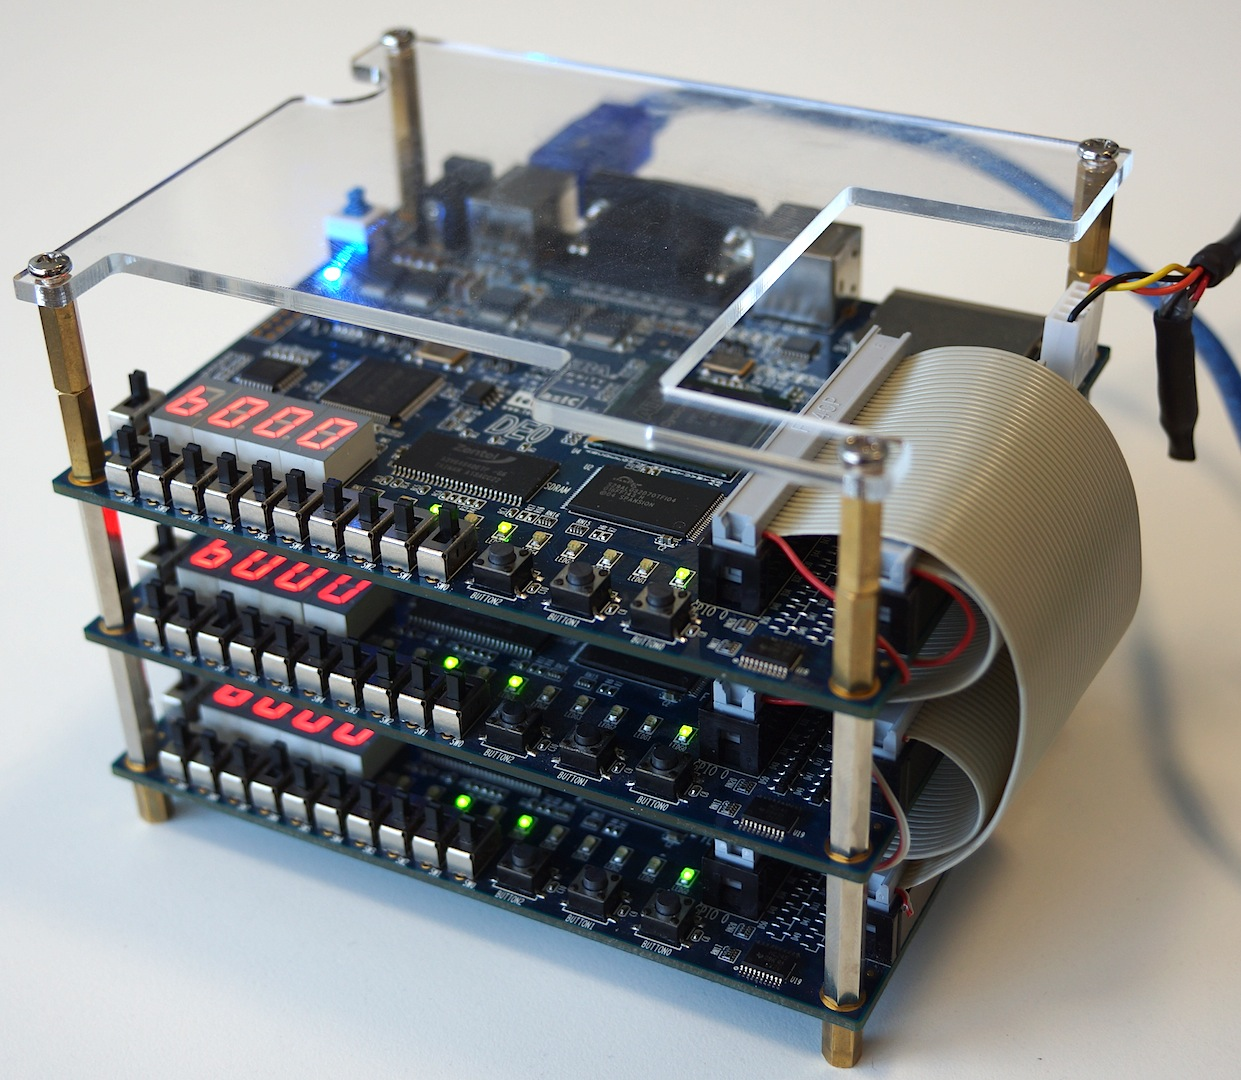
\includegraphics[width=\columnwidth]{./figs/cluster.JPG}
  \caption{Top Level Diagram, 1 Master, 2 Slave Devices}
  \label{fig:de0}
\end{figure}
\end{center}


\section{Results}

The implementation of this system has been tested both in the resource overhead associated with the input/output data transfers and the scalability of the design across many devices. 


\subsection{Resource Utilisation}
In terms of resource utilisation both memory utilisation and logic utilisation was measured when synthesising for different numbers of detection pixels and cluster size. It was important in these measurements that scalability was taken into account. 
\begin{table}
\begin{tabular}{C{0.65cm} C{0.65cm}  | C{2.5cm} C{2.5cm} }% centered columns (4 columns)
\hline\hline %inserts double horizontal lines 
Pixel Count & Cluster Size & Logic Elements (Master) (Slave) & Memory Bits (Master) (Slave) \\
\hline 
% inserts single horizontal line
9 &  3 & (5,808)~(5,175) & (5,620)~(4,532)\\
15 & 3 & (7,946)~(8,230) & (6,612)~(4,732)\\
27 & 3 & (14,097)~(14,021) & (8,908)~(5,140)\\
45 & 3 & (21,701)~(26,448) & (12,124)~(5,740)\\
99 & 3 & (44,825)~(48,578) & (22,732)~(7,548)\\
\hline 
40 & 1 & (58,609)~(N/A)~~~ & (13,896)~(N/A)\\
40 & 2 & (28,284)~(26,957) & (11,904)~(6,240)\\
40 & 4 & (15,084)~(14,116) & (10,888)~(5,240)\\
40 & 5 & (12,623)~(10,931) & (10,696)~(5,040)\\
40 & 8 & (8,799)~(7,735) & (10,420)~(4,740)\\
40 & 10 & (7,442)~(5,958) & (10,336)~(4,640)\\
\hline
\end{tabular}
\caption{Resource Utilisation}
\label{tab:res}
\end{table}
Figure \ref{tab:res} shows that the resource utilisation of this design scales linearly with pixel count with a small constant resource utilisation. This constant offset of around 5,000 logic elements per device is the full logic element cost of all the data transfer logic. The memory utilisation also scales linearly with pixel count and number of devices, however it can be seen the memory utilisation is of the same order of magnitude as the logic elements used. For common FPGA devices produced today memory resources are significantly more abundant than logic elements and as such the memory never becomes a limiting factor even when caching all read data on chip.

These results were produced by running synthesis on code in Quartus 13.0 build 156 for Altera Cyclone III devices. These results show that the host interface logic is responsible for a constant 4,000 logic elements, above this the logic count scales linearly with pixel count on both the master and slave devices. The scaling in terms of cluster size shows that the interface logic is present on each device, so a small incentive in favour of a small number of powerful devices is found. This effect is compounded by the clock skew that is found by using larger numbers of devices as discussed below. It must be noted here that library size scales badly, this is because the library must only store the best results found by the comparison engine, this results in all the library entries being compared each cycle which is highly complex. It is important to note however, that library size should be set by the duplication of DNA performed during detection and is therefore unlikely to scale to larger sizes. 

The memory utilisation also scales linearly with problem size, however the absolute values of memory utilisation are orders of magnitude smaller than the memory available on a normal device so do not become a limiting factor.



\subsection{Design Scalability}

As covered in the resource utilisation section the logic utilisation scales linearly with pixel count, and spreads logic evenly across all devices in the cluster. An important limiting factor is the library size, the library size is directly effected by the coverage of the DNA seqeunce. Due to design choices made in the design of each pixel the library maps primarily to logic cells instead of memory bits. As a result memory utilisation is relatively low, often utilising less than 3\% of device memory resources and comparison speed is higher. 

There are two further limitations to the design scalability of this architecture; the first being the practical clock synchronisation limits, and the second being the processing delay introduced to the algorithm by inter-FPGA communications. 

Due to the synchronisation of data between devices each extra device requires a 2 clock cycle delay to be added to each comparison cycle. This means that whilst more pixels can be added, the existing pixels run marginally slower, this produces an effect which diminishes the returns on added extra hardware as shown in figure \cite{fig:scale}.




\begin{figure}[!h]
  \centering
  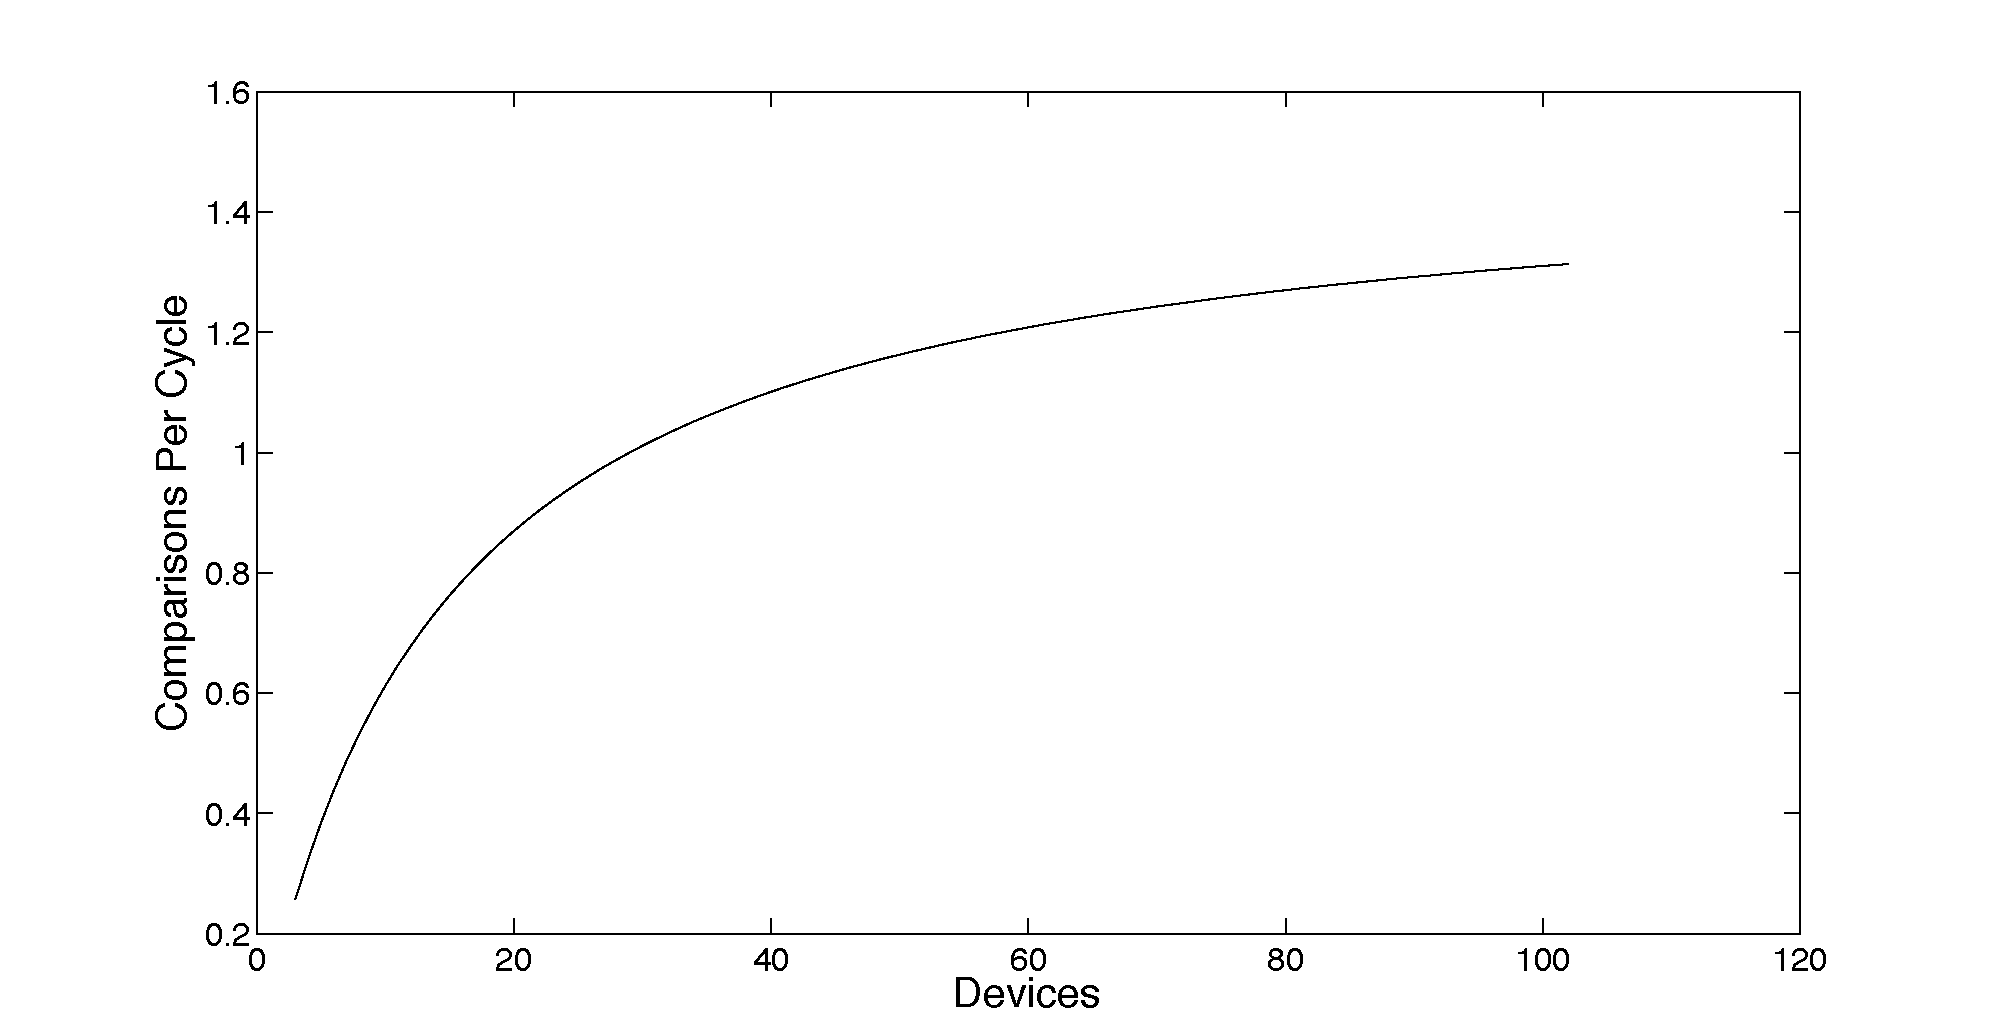
\includegraphics[width=0.9\columnwidth]{./figs/scalability.pdf}
  \caption{Scaling of Algorithm Speed with Cluster Size}
    \label{fig:scale}
\end{figure}

\subsection{Application to Large Problem Sizes}

The design of the pixel-based algorithm is such that an all-against-all comparison can only be executed in a symmetrical way, where every pixel is compared only against strings that have their own local pixels. This can be considered in matrix form, where hte algorithm is only capable of peforming a square matrix of comparisons with each entry in the matrix representing the row's string compared to the columns's string. A limitation of this algorithm therefore, is that larger comparison matrices cannot be decomposed into non-overlapping square submatrices that can be computed with this algorithm, only the leading diagonal of the larger matrix can be computed without duplicated effort. For this reaosn the algorithm is limited to comparisons with only the number of input strings equal to the number of computational pixels. A future development of this algorithm could however, break the ring network loop and feed in extra data, allowing for an arbitrary sized rectangular matrix of comparisons to be performed. This would allow non-dunplication of work with only minor modifications to the core algorithm.
% Reminder: the "draftcls" or "draftclsnofoot", not "draft", class option
% should be used if it is desired that the figures are to be displayed while
% in draft mode.

% An example of a floating figure using the graphicx package.
% Note that \label must occur AFTER (or within) \caption.
% For figures, \caption should occur after the \includegraphics.
%
%\begin{figure}
%\centering
%\includegraphics[width=2.5in]{myfigure}
% where an .eps filename suffix will be assumed under latex, 
% and a .pdf suffix will be assumed for pdflatex
%\caption{Simulation Results}
%\label{fig_sim}
%\end{figure}


% An example of a double column floating figure using two subfigures.
%(The subfigure.sty package must be loaded for this to work.)
% The subfigure \label commands are set within each subfigure command, the
% \label for the overall fgure must come after \caption.
% \hfil must be used as a separator to get equal spacing
%
%\begin{figure*}
%\centerline{\subfigure[Case I]{\includegraphics[width=2.5in]{subfigcase1}
% where an .eps filename suffix will be assumed under latex, 
% and a .pdf suffix will be assumed for pdflatex
%\label{fig_first_case}}
%\hfil
%\subfigure[Case II]{\includegraphics[width=2.5in]{subfigcase2}
% where an .eps filename suffix will be assumed under latex, 
% and a .pdf suffix will be assumed for pdflatex
%\label{fig_second_case}}}
%\caption{Simulation results}
%\label{fig_sim}
%\end{figure*}



% An example of a floating table. Note that, for IEEE style tables, the 
% \caption command should come BEFORE the table. Table text will default to
% \footnotesize as IEEE normally uses this smaller font for tables.
% The \label must come after \caption as always.
%
%\begin{table}
%% increase table row spacing, adjust to taste
%\renewcommand{\arraystretch}{1.3}
%\caption{An Example of a Table}
%\label{table_example}
%\begin{center}
%% Some packages, such as MDW tools, offer better commands for making tables
%% than the plain LaTeX2e tabular which is used here.
%\begin{tabular}{|c||c|}
%\hline
%One & Two\\
%\hline
%Three & Four\\
%\hline
%\end{tabular}
%\end{center}
%\end{table}


\section{Conclusion}
In conclusion, a small FPGA cluster has shown as a proof of concept that considerable processing work can be passed off in the DNA sequencing tool-chain. The logic utilisation scaled linearly with problem size and split computation evenly across multiple devices. At the small scale that this work was completed on, no speed-up was achieved over software based approaches, however the code has been shown to scale well and the key speed-ups would be seen as problem size increases. This solution also shows significant promise in direct integration into a detection tool-chain using the sequencing process to mask the processing time of the comparison engine. Due to the way the design scaled it was shown that small clusters of high power devices would be the ideal way of producing the most processing power.

% conference papers do not normally have an appendix

% use section* for acknowledgement
%\section*{Acknowledgment}
% optional entry into table of contents (if used)
%\addcontentsline{toc}{section}{Acknowledgment}
%The authors would like to thank...

% trigger a \newpage just before the given reference
% number - used to balance the columns on the last page
% adjust value as needed - may need to be readjusted if
% the document is modified later
%\IEEEtriggeratref{8}
% The "triggered" command can be changed if desired:
%\IEEEtriggercmd{\enlargethispage{-5in}}

% references section
% NOTE: BibTeX documentation can be easily obtained at:
% http://www.ctan.org/tex-archive/biblio/bibtex/contrib/doc/

% can use a bibliography generated by BibTeX as a .bbl file
% standard IEEE bibliography style from:
% http://www.ctan.org/tex-archive/macros/latex/contrib/supported/IEEEtran/bibtex
%\bibliographystyle{IEEEtran.bst}
% argument is your BibTeX string definitions and bibliography database(s)
%\bibliography{IEEEabrv,../bib/paper}
%
% <OR> manually copy in the resultant .bbl file
% set second argument of \begin to the number of references
% (used to reserve space for the reference number labels box)


% that's all folks
\end{document}


